\documentclass[noback]{cuposter}

%%\documentclass[noback,portrait]{cuposter}
%% To make a poster in portrait, use the "portrait" option to
%% documentclass as shown above.

\usepackage{mathptmx}
\usepackage{xspace}
\usepackage{amsmath}
\usepackage{pifont}
\usepackage{psfrag}
\usepackage{graphicx}

\usepackage{wrapfig}


\begin{document}

%% Not needed for most posters.
%%\renewcommand{\poster@ancimage}{/tmp/empty.ps}
\newcommand{\don}{\ensuremath{d_{\textsc{ON}}}}
\newcommand{\doff}{\ensuremath{d_{\textsc{OFF}}}}
\newcommand{\dsoma}{\ensuremath{d_{\textsc{SOMA}}} \xspace}
\newcommand{\um}{\ensuremath{\mu \text{m}}\xspace}
\newcommand{\dmin}{d$_{\textup{min}}$\xspace}

\title{How to make a full body 3D scanner}
%%\subtitle{The poster subtitle here}
\author{Emile Okada$^1$, Supervisors: Carola Schoenlieb$^1$, Martin Benning$^1$, Matthias Ehrhardt$^1$, Veronica Corona$^1$}
\address{$^1$University of Cambridge}

\makeposter

\section{Introduction}
Have you ever wanted a statue of yourself, but never had the 3D scanner for the job? 
In this poster I'll be detailing the maths behind reconstructing 3D objects from their projections and some of the challenges I faced trying to actually make such a scanner myself.

%\vspace*{-3cm}
\section{Reconstruction from projections}
Let $D$ be a subset of the plane.
In this project we consider the projections corresponding to the shadow of the object caused by incident light rays coming in at an angle $\theta$ to the horizontal.

\vspace*{2cm}
{
\centerline{
\includegraphics[width=12cm]
  {figs/shadow_1.ps}}
}
\vspace*{5mm} \textbf{Figure 1}: \textit{Shadow of $D$ from light rays incident at an angle $\theta$.}

Consider the region $D_{\theta}$ corresponding to the union of all light rays blocked by the region $D$.
In the case of Fig. 1, this region looks like Fig. 2.

\vspace*{2cm}
{
\centerline{
\includegraphics[width=12cm]
  {figs/shadow_2.ps}}
}
\vspace*{5mm} \textbf{Figure 2}: \textit{The region $D_{\theta}$ corresponding to the projection in Fig. 1.}

Note in particular that $D\subset D_{\theta}$. 
It follows that for any subset $I\subset[0,2\pi]$, $D\subset \cap_{\alpha\in I}D_{\alpha}$.
When the set $I$ is finite, $\cap_{\alpha\in I}D_{\alpha}$ is a bounding polygon of $D$ and is what we'll use as our reconstruction.
It is interesting to note that this reconstruction is exact if $I = [0,2\pi]$ and $D$ is convex.
This is an immediate consequence of the fact that if $D$ convex then it is the intersection of all its supporting hyperplanes.

We now wish to extend this approach to 3D objects.
The way we do it is that we simply reconstruct cross sections of the object.
Consider the following bunny.

\vspace*{2cm}
{
\centerline{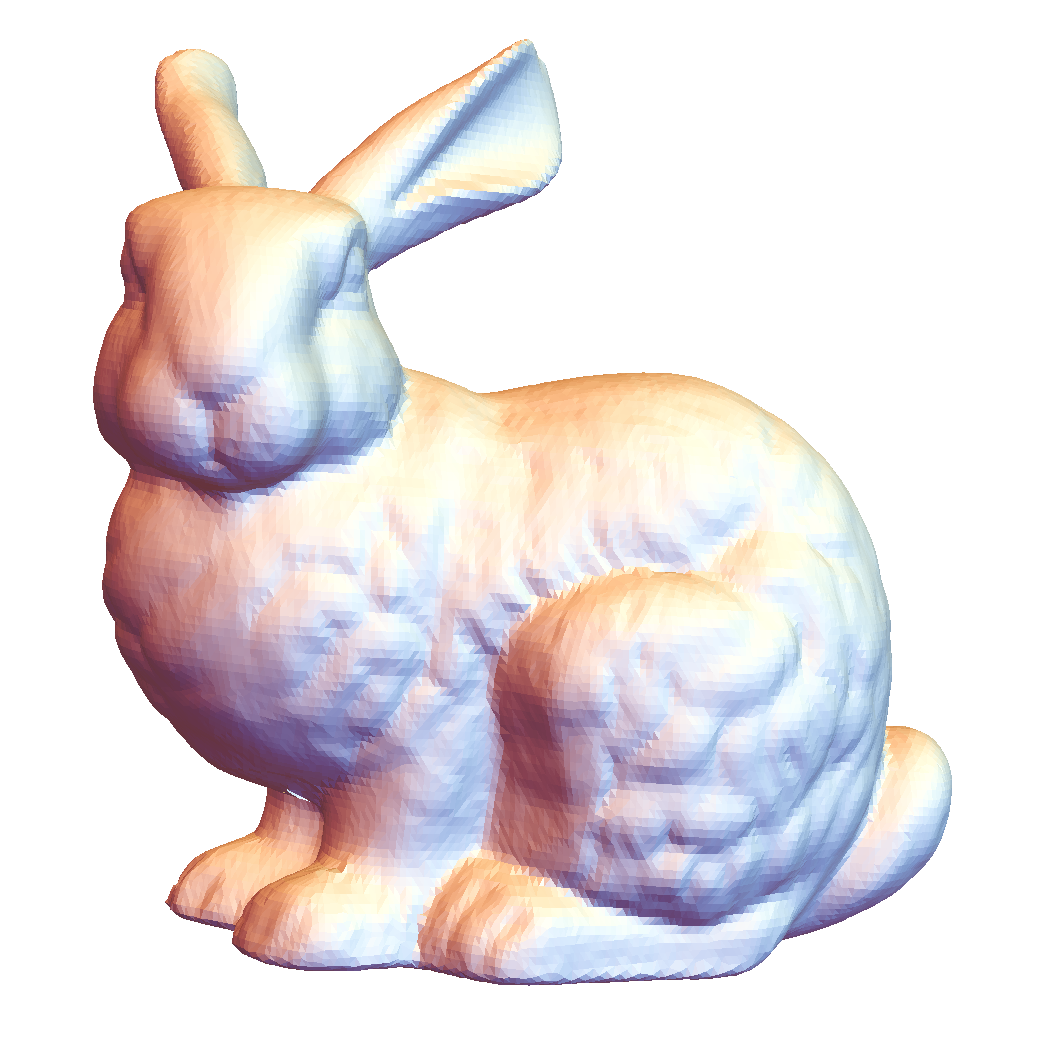
\includegraphics[width=12cm]
  {figs/3D_rabit.ps}}
}
\vspace*{5mm} \textbf{Figure 3}: \textit{3D rabit.}

In the 3D case we project the shadows onto a plane, and rotate the rabit about the z-axis to get different angles.
The shadow of the rabit with $\theta=\pi$ is shown in Fig. 4.

\vspace*{-1cm}
{
\centerline{
\includegraphics[width=22cm]
  {figs/1.ps}}
}
\vspace*{-1cm} \textbf{Figure 4}: \textit{Shadow of rabit with $\theta=\pi$.}

We then reduce the problem to the 2D case by treating each row of the image as the shadow of a 2D region.
We can then piece together all the reconstructed cross sections to get the 3D object.

\vspace*{2cm}
{
\centerline{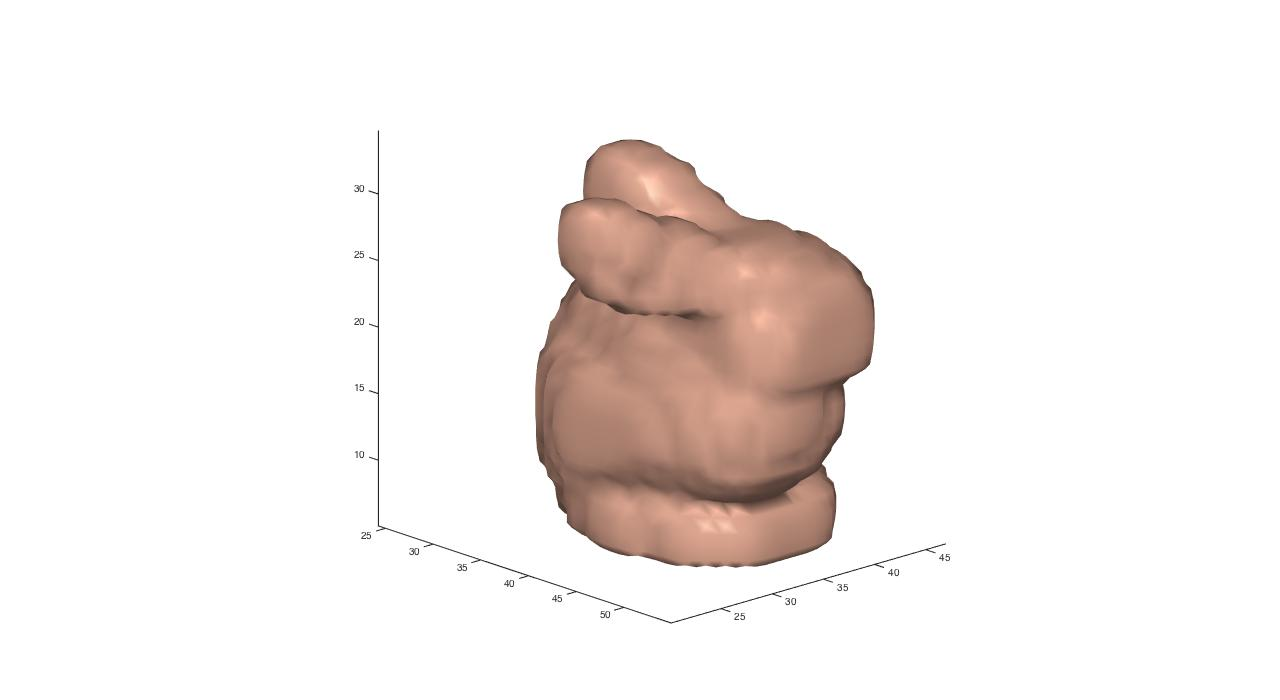
\includegraphics[width=22cm]
  {figs/rabit_surface_1.ps}}
}
\vspace*{5mm} \textbf{Figure 5}: \textit{Reconstructed rabit.}

\vspace*{-10mm} 

\section{Construction}
As a mathematician, the constuction part turned out to be by far the most challenging part of the project.
The set up consisted of a LED floodlight casting the shadow of the subject onto a large shadow screen with a webcam behind to capture images.
The subject stood on a turntable which rotated them around.

\vspace*{2cm}
{
\centerline{\includegraphics[width=18cm]
  {figs/set_up.ps}}
}
\vspace*{5mm} \textbf{Figure 6}: \textit{The setup.}

With no prior engineering experience however, I underestimated the amount of time it would take to make the turntable and so did not have time to make the last bit of the circuit that was meant to accurately determine how many degrees the turntable had turned.
Without this bit I had to rely on a significantly less accurate timer based solution.
Nonetheless, we got some results as can be seen in Fig. 7, and the hope is to finish the circuitry by easter.

\vspace*{2cm}
{
\centerline{\includegraphics[width=18cm]
  {figs/results.ps}}
}
\vspace*{5mm} \textbf{Figure 7}: \textit{3D scan of my supervisor.}


\end{document}

% LocalWords:  RGCs
